% Use chapters in the appendix
% Appendix A: Performance parameters, notebook
% Appendix B: Additional tables, for quantification results



% Appendix A: Performance parameters, notebook
\chapter{Notebook: Performance parameters}
\label{appendix:performance}

This is the notebook for the SEM EDS performance parameters.
The notebook is available \href{https://github.com/brynjarmorka/sem-eds-qc/blob/main/healthcheck.ipynb}{on GitHub through this link}\footnote{\url{https://github.com/brynjarmorka/sem-eds-qc/blob/main/healthcheck.ipynb}}. 
The notebooks and code for the quantification and bulk corrections are located in the GitHub repository \href{https://github.com/brynjarmorka/eds-sem-bulk-corrections}{"eds-sem-bulk-corrections"}, under the user "brynjarmorka".
The notebook below have headers which are listed in \cref{method:data_treatment:notebook}.
The example spectrum run through in the notebook is the GaSb spectrum with $30$ kV, $50$ pA, and PT $6$.

\newgeometry{left=1.5cm,right=1.5cm,bottom=1.5cm, top=1.0cm} % change the margins to fit the table.
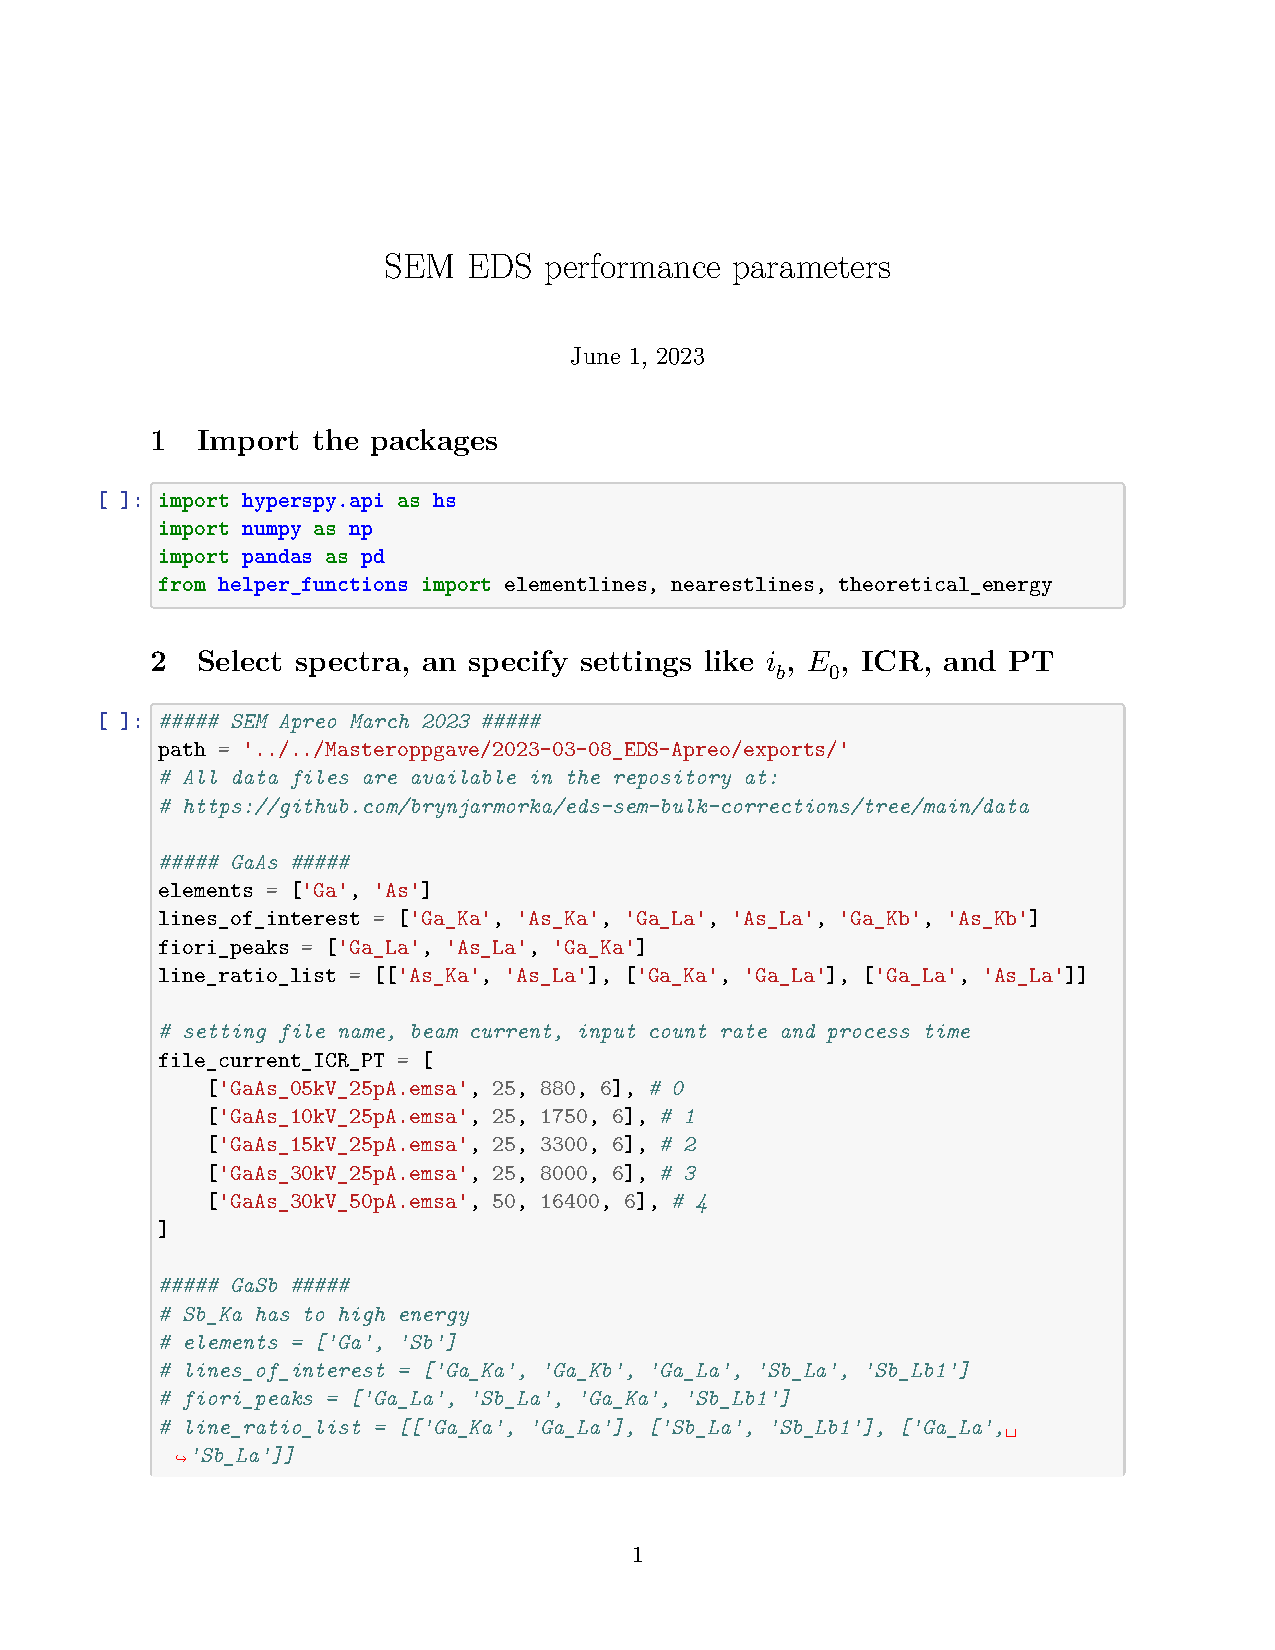
\includepdf[pages=-, pagecommand={}, width=\textwidth]{chapters/SEM EDS performance parameters.pdf}
\restoregeometry % put the margins back to normal








% Appendix B: Additional tables, for quantification results
\chapter{Quantification result tables}
\label{appendix:tables}

This appendix contains the following tables:

\begin{itemize}
    \item \cref{tab:results:TEM_quantification} - Quantification of SEM EDS data with the thin film assumption.
    \item \cref{tab:results:ZAF_corrections_range_r} - The calculated range of electrons, $r$, where the electrons still have enough energy to excite the listed X-ray line.
    \item \cref{tab:results:ZAF_corrections_factors} - The absorption correction factors for the ZAF model.
    \item \cref{tab:results:ZAF_corrections_compositions} - Quantification of SEM EDS data with the ZAF absorption correction.
    \item \cref{tab:results:XPP_compositions} - Quantification of SEM EDS data with the corrections form the XPP model.    
\end{itemize}

The table with initial quantification, i.e. from AZtec and the intensity ratio method, is given in \cref{tab:results:initial_quantification}.


\newgeometry{left=1.5cm,right=1.5cm,bottom=2.5cm, top=1.5cm} % change the margins to fit the table.
\begin{table}[phtb]
    \begin{center}
        \caption{
            Quantification of SEM EDS data with the thin film assumption, i.e. TEM EDS routines.
            Compositions in at\% from AZtec and the CL method in HyperSpy. CL* is without corrections, the others have absorption corrections with thicknesses $t$, in nm.
            The calculated k-factors from AZtec is also tabulated. 
            The table is summarized in \cref{tab:results:TEM_quantification_stats}.
            Each spectrum has two lines in the table.
        }
        %\renewcommand*{\arraystretch}{1.4}
        \label{tab:results:TEM_quantification}
        \begin{tabular}{rrrrrrrrrrrrrr}
            \hline
            \textbf{Gr.} & \textbf{Line} & \textbf{$E_0$} & \textbf{$i_b$} & \textbf{PT} & \textbf{k-factor} & \textbf{AZtec TEM} & \textbf{CL*} & \textbf{CL}   & \textbf{CL}    & \textbf{CL}    & \textbf{CL}    & \textbf{CL}   & \textbf{CL}    \\
            \emph{}      & \emph{}       & \emph{[kV]}    & \emph{[pA]}    & \emph{}     & \emph{}           & \emph{at\%}    & \emph{}      & \emph{$t$=50} & \emph{$t$=100} & \emph{$t$=200} & \emph{$t$=400} & \emph{$t$=1k} & \emph{$t$=10k} \\
            \hline
            A            & As L$\alpha$  & 5              & 25             & 6           & 1.21              & 45             & 45           & 47            & 48             & 51             & 54             & 60            & 63             \\
            A            & Ga L$\alpha$  & 5              & 25             & 6           & 1.09              & 55             & 55           & 53            & 52             & 49             & 46             & 40            & 37             \\
            A            & Ga L$\alpha$  & 10             & 25             & 6           & 1.31              & 42             & 42           & 43            & 45             & 47             & 51             & 57            & 61             \\
            A            & As L$\alpha$  & 10             & 25             & 6           & 1.22              & 58             & 58           & 57            & 55             & 53             & 49             & 43            & 39             \\
            A            & As L$\alpha$  & 15             & 25             & 6           & 1.33              & 38             & 37           & 39            & 40             & 43             & 47             & 53            & 58             \\
            A            & Ga L$\alpha$  & 15             & 25             & 6           & 1.26              & 62             & 63           & 61            & 60             & 57             & 53             & 47            & 42             \\
            A            & As K$\alpha$  & 30             & 25             & 6           & 4.19              & 42             & 42           & 42            & 42             & 42             & 42             & 43            & 50             \\
            A            & Ga K$\alpha$  & 30             & 25             & 6           & 3.27              & 58             & 58           & 58            & 58             & 58             & 58             & 57            & 50             \\
            A            & As K$\alpha$  & 30             & 50             & 6           & 4.19              & 42             & 41           & 42            & 42             & 42             & 42             & 43            & 50             \\
            A            & Ga K$\alpha$  & 30             & 50             & 6           & 3.27              & 58             & 59           & 59            & 58             & 58             & 58             & 57            & 50             \\
            \hline
            B            & Ga L$\alpha$  & 5              & 50             & 6           & 1.09              & 91             & -            & -             & -              & -              & -              & -             & -              \\
            B            & Sb M$\zeta$    & 5              & 50             & 6           & 0.96              & 9              & -            & -             & -              & -              & -              & -             & -              \\
            B            & Ga L$\alpha$  & 10             & 50             & 6           & 1.22              & 42             & 52           & 55            & 58             & 62             & 67             & 76            & 85             \\
            B            & Sb L$\alpha$  & 10             & 50             & 6           & 3.30              & 58             & 48           & 45            & 42             & 38             & 33             & 24            & 15             \\
            B            & Ga L$\alpha$  & 15             & 50             & 6           & 1.26              & 29             & 39           & 42            & 45             & 49             & 56             & 67            & 80             \\
            B            & Sb L$\alpha$  & 15             & 50             & 6           & 2.75              & 71             & 61           & 58            & 55             & 51             & 44             & 33            & 20             \\
            B            & Ga K$\alpha$  & 30             & 50             & 6           & 3.27              & 45             & 57           & 56            & 56             & 56             & 55             & 53            & 36             \\
            B            & Sb L$\alpha$  & 30             & 50             & 6           & 2.32              & 55             & 43           & 44            & 44             & 44             & 45             & 47            & 64             \\
            \hline
            C            & Ga K$\alpha$  & 30             & 50             & 4           & 3.27              & 45             & 57           & 57            & 57             & 56             & 55             & 53            & 36             \\
            C            & Sb L$\alpha$  & 30             & 50             & 4           & 2.32              & 55             & 43           & 43            & 43             & 44             & 45             & 47            & 64             \\
            C            & Ga K$\alpha$  & 30             & 50             & 2           & 3.27              & 45             & 58           & 58            & 57             & 57             & 56             & 54            & 37             \\
            C            & Sb L$\alpha$  & 30             & 50             & 2           & 2.32              & 55             & 42           & 42            & 43             & 43             & 44             & 46            & 63             \\
            C            & Ga K$\alpha$  & 30             & 50             & 1           & 3.27              & 45             & 59           & 59            & 59             & 58             & 57             & 55            & 38             \\
            C            & Sb L$\alpha$  & 30             & 50             & 1           & 2.32              & 55             & 41           & 41            & 41             & 42             & 43             & 45            & 62             \\
            \hline
            D            & Ga L$\alpha$  & 15             & 200            & 6           & 1.26              & 29             & 38           & 41            & 44             & 49             & 56             & 67            & 79             \\
            D            & Sb L$\alpha$  & 15             & 200            & 6           & 2.75              & 71             & 62           & 59            & 56             & 51             & 44             & 33            & 21             \\
            D            & Ga L$\alpha$  & 15             & 400            & 6           & 1.26              & 29             & 38           & 41            & 44             & 49             & 56             & 67            & 79             \\
            D            & Sb L$\alpha$  & 15             & 400            & 6           & 2.75              & 71             & 62           & 59            & 56             & 51             & 44             & 33            & 21             \\
            D            & Ga K$\alpha$  & 30             & 400            & 1           & 3.27              & 45             & 59           & 58            & 58             & 58             & 57             & 55            & 37             \\
            D            & Sb L$\alpha$  & 30             & 400            & 1           & 2.32              & 55             & 41           & 42            & 42             & 42             & 43             & 45            & 63             \\
            \hline
        \end{tabular}
    \end{center}
\end{table}
\restoregeometry % put the margins back to normal

\newgeometry{top=1.5cm} % change the margins to fit the table.
\begin{table}[p]
    \begin{center}
        \caption{
            Selected maximum ranges of creation for lines in different specimen, based on the Kanaya-Okayama parameterization.
            The path length of the X-rays are $r \cdot \csc(TOA)$.
            The ranges are used to calculate the ZAF absorption correction factors, listed in \cref{tab:results:ZAF_corrections_factors}.
        }
        %\renewcommand*{\arraystretch}{1.4}
        \label{tab:results:ZAF_corrections_range_r}
        \begin{tabular}{rrrrrr}
            \hline
            \textbf{Specimen} & \textbf{Line} & \textbf{$r$ at 30 kV} & \textbf{$r$ at 15 kV} & \textbf{$r$ at 10 kV} & \textbf{$r$ at 5 kV} \\
            \emph{}           & \emph{}       & \emph{[\textmu m]}    & \emph{[\textmu m]}    & \emph{[\textmu m]}    & \emph{[\textmu m]}   \\
            \hline
            GaAs              & Ga L$\alpha$  & 4.13                  & 1.29                  & 0.65                  & 0.19                 \\
                              & As L$\alpha$  & 4.12                  & 1.28                  & 0.64                  & 0.19                 \\
                              & Ga K$\alpha$  & 3.56                  & 0.72                  & 0.08                  & -                    \\
            %&As K$\alpha$&&&&\\
            \hline
            GaSb              & Ga L$\alpha$  & 4.02                  & 1.25                  & 0.63                  & 0.19                 \\
                              & Sb L$\alpha$  & 3.92                  & 1.15                  & 0.53                  & 0.09                 \\
            %&Ga K$\alpha$&&&&\\
            \hline
        \end{tabular}
    \end{center}
\end{table}


\begin{table}[p]
    \begin{center}
        \caption{
            Absorption correction factors ($A$) from the ZAF method used.
            The absorption correction factors are in the three rightmost columns, indicated by "$A$ r/x", where x is the number that the maximum electron range is divided by.
            %Some of the $r$ values are tabluated in \cref{tab:results:ZAF_corrections_range_r}.
            Similar specimen, line, and $E_0$ have the same $A$, thus the $15$ kV and $30$ kV GaSb $A$-factors are grouped together.
        }
        %\renewcommand*{\arraystretch}{1.4}
        \label{tab:results:ZAF_corrections_factors}
        \begin{tabular}{rrrrrr}
            \hline
            \textbf{Groups} & \textbf{Line} & \textbf{$E_0$} & \textbf{$A$ with r/2} & \textbf{$A$ with r/3} & \textbf{$A$ with r/4} \\
            \emph{}         & \emph{}       & \emph{[kV]}    & \emph{}               & \emph{}               & \emph{}               \\
            \hline
            A               & As L$\alpha$  & 5              & 1.41                  & 1.26                  & 1.19                  \\
            A               & Ga L$\alpha$  & 5              & 1.14                  & 1.09                  & 1.07                  \\
            A               & As L$\alpha$  & 10             & 3.27                  & 2.20                  & 1.81                  \\
            A               & Ga L$\alpha$  & 10             & 1.58                  & 1.35                  & 1.26                  \\
            A               & As L$\alpha$  & 15             & 10.67                 & 4.85                  & 3.27                  \\
            A               & Ga L$\alpha$  & 15             & 2.48                  & 1.83                  & 1.57                  \\
            A               & As K$\alpha$  & 30             & 1.23                  & 1.15                  & 1.11                  \\
            A               & Ga K$\alpha$  & 30             & 1.08                  & 1.05                  & 1.04                  \\
            \hline
            B               & Ga L$\alpha$  & 5              & 1.64                  & 1.39                  & 1.28                  \\
            B               & Sb L$\alpha$  & 5              & 1.02                  & 1.01                  & 1.01                  \\
            B               & Ga L$\alpha$  & 10             & 5.24                  & 3.02                  & 2.29                  \\
            B               & Sb L$\alpha$  & 10             & 1.14                  & 1.09                  & 1.07                  \\
            B, D            & Ga L$\alpha$  & 15             & 27.19                 & 9.04                  & 5.21                  \\
            B, D            & Sb L$\alpha$  & 15             & 1.32                  & 1.20                  & 1.15                  \\
            B, C, D         & Ga K$\alpha$  & 30             & 1.27                  & 1.17                  & 1.13                  \\
            B, C, D         & Sb L$\alpha$  & 30             & 2.56                  & 1.87                  & 1.60                  \\
            \hline
        \end{tabular}
    \end{center}
\end{table}

\restoregeometry % put the margins back to normal


\newgeometry{top=2cm} % change the margins to fit the table.
\begin{table}[phtb]
    \begin{center}
        \caption{
            Compositions from the intensity ratio method with absorption corrected intensities. The uncorrected at.\% value is tabulated for reference.
            See \cref{tab:results:ZAF_corrections_factors} for the correction factors.
            Average numbers are given in \cref{tab:results:ZAF_corrections_compositions_stats}.
            Each spectrum has two lines in the table.
        }
        %\renewcommand*{\arraystretch}{1.4}
        \label{tab:results:ZAF_corrections_compositions}
        \begin{tabular}{rrrrrrrr}
            \hline
            \textbf{Groups} & \textbf{Line} & \textbf{$E_0$} & \textbf{$i_b$} & \textbf{Uncorr. at.\%} & \textbf{at.\% with r/2} & \textbf{at.\% with r/3} & \textbf{at.\% with r/4} \\
            \emph{}         & \emph{}       & \emph{[kV]}    & \emph{[pA]}    & \emph{}                & \emph{}                 & \emph{}                 & \emph{}                 \\
            \hline
            A               & As L$\alpha$  & 5              & 25             & 43                     & 48                      & 46                      & 45                      \\
            A               & Ga L$\alpha$  & 5              & 25             & 57                     & 52                      & 54                      & 55                      \\
            A               & As L$\alpha$  & 10             & 25             & 40                     & 58                      & 52                      & 49                      \\
            A               & Ga L$\alpha$  & 10             & 25             & 60                     & 42                      & 48                      & 51                      \\
            A               & As L$\alpha$  & 15             & 25             & 36                     & 71                      & 60                      & 54                      \\
            A               & Ga L$\alpha$  & 15             & 25             & 64                     & 29                      & 40                      & 46                      \\
            A               & As K$\alpha$  & 30             & 25             & 36                     & 39                      & 38                      & 37                      \\
            A               & Ga K$\alpha$  & 30             & 25             & 64                     & 61                      & 62                      & 63                      \\
            A               & As K$\alpha$  & 30             & 50             & 36                     & 39                      & 38                      & 37                      \\
            A               & Ga K$\alpha$  & 30             & 50             & 64                     & 61                      & 62                      & 63                      \\
            \hline
            B               & Ga L$\alpha$  & 5              & 50             & 97                     & 98                      & 98                      & 98                      \\
            B               & Sb L$\alpha$  & 5              & 50             & 3                      & 2                       & 2                       & 2                       \\
            B               & Ga L$\alpha$  & 10             & 50             & 75                     & 93                      & 89                      & 86                      \\
            B               & Sb L$\alpha$  & 10             & 50             & 25                     & 7                       & 11                      & 14                      \\
            B               & Ga L$\alpha$  & 15             & 50             & 58                     & 97                      & 91                      & 86                      \\
            B               & Sb L$\alpha$  & 15             & 50             & 42                     & 3                       & 9                       & 14                      \\
            B               & Ga K$\alpha$  & 30             & 50             & 48                     & 32                      & 37                      & 40                      \\
            B               & Sb L$\alpha$  & 30             & 50             & 52                     & 68                      & 63                      & 60                      \\
            \hline
            C               & Ga K$\alpha$  & 30             & 50             & 48                     & 32                      & 37                      & 40                      \\
            C               & Sb L$\alpha$  & 30             & 50             & 52                     & 68                      & 63                      & 60                      \\
            C               & Ga K$\alpha$  & 30             & 50             & 49                     & 33                      & 38                      & 41                      \\
            C               & Sb L$\alpha$  & 30             & 50             & 51                     & 67                      & 62                      & 59                      \\
            C               & Ga K$\alpha$  & 30             & 50             & 51                     & 34                      & 39                      & 42                      \\
            C               & Sb L$\alpha$  & 30             & 50             & 49                     & 66                      & 61                      & 58                      \\
            \hline
            D               & Ga L$\alpha$  & 15             & 200            & 57                     & 97                      & 91                      & 86                      \\
            D               & Sb L$\alpha$  & 15             & 200            & 43                     & 3                       & 9                       & 14                      \\
            D               & Ga L$\alpha$  & 15             & 400            & 57                     & 97                      & 91                      & 86                      \\
            D               & Sb L$\alpha$  & 15             & 400            & 43                     & 3                       & 9                       & 14                      \\
            D               & Ga K$\alpha$  & 30             & 400            & 50                     & 33                      & 39                      & 41                      \\
            D               & Sb L$\alpha$  & 30             & 400            & 50                     & 67                      & 61                      & 59                      \\
            %
            %E&Map&&&&&&\\
            %E&Map&&&&&&\\
            %&&&&&&&\\
            \hline
        \end{tabular}
    \end{center}
\end{table}
\restoregeometry % put the margins back to normal

\newgeometry{top=2cm} % change the margins to fit the table.
\begin{table}[phtb]
    \begin{center}
        \caption{
            Compositions from the area ratio method XPP corrections.
            Two type of corrections have been tested where the measured intensity $I_A$ of each peak have been divided by (1) the peaks absorption correction factor $f(\chi)$, and (2) by the peaks area $F$ of the $\phi(\rho z)$ curve.
            $f(\chi)$ is defined in \cref{eq:theory:quantitative:pap:absorption_correction}, and $F$ is defined in \cref{eq:theory:quantitative:pap:general_principle:F}.
        }
        %\renewcommand*{\arraystretch}{1.4}
        \label{tab:results:XPP_compositions}
        \begin{tabular}{rrrrrrrr}
            \hline
            \textbf{Groups} & \textbf{Line} & \textbf{$E_0$} & \textbf{$i_b$} & \textbf{Uncorr. area ratio} & \textbf{XPP corr. $(I_A/f(\chi))$} & \textbf{XPP corr. $(I_A/F)$} \\
            \emph{}         & \emph{}       & \emph{[kV]}    & \emph{[pA]}    & \emph{[at\%]}               & \emph{[at\%]}                      & \emph{[at\%]}                \\
            \hline
            A               & As L$\alpha$  & 5              & 25             & 43                          & 43                                 & 44                           \\
            A               & Ga L$\alpha$  & 5              & 25             & 57                          & 57                                 & 56                           \\
            A               & As L$\alpha$  & 10             & 25             & 40                          & 42                                 & 41                           \\
            A               & Ga L$\alpha$  & 10             & 25             & 60                          & 58                                 & 59                           \\
            A               & As L$\alpha$  & 15             & 25             & 36                          & 39                                 & 36                           \\
            A               & Ga L$\alpha$  & 15             & 25             & 64                          & 61                                 & 64                           \\
            A               & As K$\alpha$  & 30             & 25             & 36                          & 36                                 & 37                           \\
            A               & Ga K$\alpha$  & 30             & 25             & 64                          & 64                                 & 63                           \\
            A               & As K$\alpha$  & 30             & 50             & 36                          & 36                                 & 37                           \\
            A               & Ga K$\alpha$  & 30             & 50             & 64                          & 64                                 & 63                           \\
            \hline
            B               & Ga L$\alpha$  & 5              & 50             & 97                          & 97                                 & 91                           \\
            B               & Sb L$\alpha$  & 5              & 50             & 3                           & 3                                  & 9                            \\
            B               & Ga L$\alpha$  & 10             & 50             & 75                          & 79                                 & 65                           \\
            B               & Sb L$\alpha$  & 10             & 50             & 25                          & 21                                 & 35                           \\
            B               & Ga L$\alpha$  & 15             & 50             & 58                          & 67                                 & 50                           \\
            B               & Sb L$\alpha$  & 15             & 50             & 42                          & 33                                 & 50                           \\
            B               & Ga K$\alpha$  & 30             & 50             & 48                          & 48                                 & 56                           \\
            B               & Sb L$\alpha$  & 30             & 50             & 52                          & 52                                 & 44                           \\
            \hline
            C               & Ga K$\alpha$  & 30             & 50             & 48                          & 48                                 & 56                           \\
            C               & Sb L$\alpha$  & 30             & 50             & 52                          & 52                                 & 44                           \\
            C               & Ga K$\alpha$  & 30             & 50             & 49                          & 49                                 & 57                           \\
            C               & Sb L$\alpha$  & 30             & 50             & 51                          & 51                                 & 43                           \\
            C               & Ga K$\alpha$  & 30             & 50             & 51                          & 50                                 & 58                           \\
            C               & Sb L$\alpha$  & 30             & 50             & 49                          & 50                                 & 42                           \\
            \hline
            D               & Ga K$\alpha$  & 30             & 400            & 50                          & 50                                 & 58                           \\
            D               & Sb L$\alpha$  & 30             & 400            & 50                          & 50                                 & 42                           \\
            D               & Ga L$\alpha$  & 15             & 200            & 57                          & 66                                 & 49                           \\
            D               & Sb L$\alpha$  & 15             & 200            & 43                          & 34                                 & 51                           \\
            D               & Ga L$\alpha$  & 15             & 400            & 57                          & 66                                 & 49                           \\
            D               & Sb L$\alpha$  & 15             & 400            & 43                          & 34                                 & 51                           \\
            \hline
        \end{tabular}
    \end{center}
\end{table}
\restoregeometry % put the margins back to normal


